\documentclass[tikz,border=5mm]{standalone}
\usepackage{tikz}
\usetikzlibrary{calc}

\begin{document}
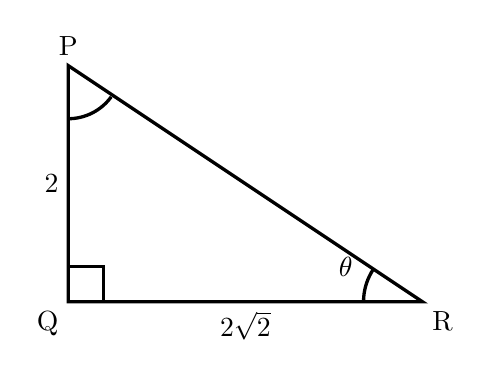
\begin{tikzpicture}[scale=1.5]

% Define vertices
\coordinate (P) at (0,2);
\coordinate (Q) at (0,0);
\coordinate (R) at (3,0);

% Draw triangle PQR
\draw[very thick] (P) -- (Q) -- (R) -- cycle;

% Draw right angle mark at Q
\draw[very thick] (Q) ++(0.3,0) -- ++(0,0.3) -- ++(-0.3,0);

% Angle arc at P (inside triangle)
% Starts pointing down (-90°) toward Q, ends pointing toward R
\draw[very thick] ($(P)+(0,-0.45)$) arc[start angle=-90, end angle=-36, radius=0.45];

% Angle arc at R (θ) - inside the triangle
% Starts pointing left (180°) toward Q, ends pointing toward P
\draw[very thick] ($(R)+(-0.5,0)$) arc[start angle=180, end angle=146, radius=0.5];
\node at ($(R)+(-0.65,0.3)$) {\normalsize $\theta$};

% Vertex labels
\node[above] at (P) {P};
\node[below left] at (Q) {Q};
\node[below right] at (R) {R};

% Side labels
\node[left] at ($(P)!0.5!(Q)$) {2};
\node[below] at ($(Q)!0.5!(R)$) {$2\sqrt{2}$};

\end{tikzpicture}
\end{document}